\chapter{Analysis techniques}

\intro{This chapter introduces the necessary toolset to perform the analyses within this thesis. It is organized to follow the common steps of the analyses. First, the generation of simulated events is introduced. Then, details of the top quark reconstruction, the employed multivariate analysis technique, and the template fit is given which are used to estimate the amount of single top quark events within the recorded data. Lastly, the partonic and fiducial objects are defined to which the observed data is unfolded to for comparison with theoretical predictions.}

%##############################################
\section{Event generation}
%##############################################
\label{sec:technique-event-gen}

To compare reconstructed data with theoretical predictions, samples of simulated events are generated from theory and passed through a simulation of the \gls{cms} detector and emulation of its readout. The standard so-called ``FullSimulation'' package~\cite{1742-6596-396-2-022003,1742-6596-664-7-072022} is based on the Geant4 toolkit~\cite{Agostinelli2003250} which provides a detailed simulation of particle trajectories and interactions with the detector material. A fast alternative, the so-called ``FastSimulation'' package, exists within \gls{cms} as well~\cite{fsimRahmat} but has not been used for simulating the detector response in the analyses within this thesis.

The event generation starts with the \glshere{me} of a hard scattering process of interest. \glshere{mc} methods are employed to sample the corresponding cross section integral. The advantage of \gls{mc}-based methods is that the variance of their result decreases as $1/n$ independently of the integral's dimensionality leading to an efficient convergence compared to quadrature-based methods~(e.g. Simpson's rule, Newton-Cotes). A common method to integrate cross sections is given by the \gls{vegas} algorithm~\cite{OHL199913}. It is based on importance sampling where the integral is sampled not uniformly but along an adaptive importance function instead. The resulting sample of events reflects the probability distribution of a process over its phase space. Typically a reweighting is performed in addition such that all events contribute the same probability (e.i. they carry the same absolute weight). 

After obtaining events from the hard interaction, a \glshere{ps} program simulates the hadronization of final state partons. In addition, the radiation of gluons or quarks from initial or final state partons is accounted for as well as contributions from soft secondary interactions, the so-called underlying event, and potential color reconnection effects. A sketch of various parts within an exemplary pp collision event after hadronization is shown in Fig.~\ref{fig:technique-mcevent}. The \gls{ps} simulation is based on Altarelli-Parisi splitting functions~\cite{Altarelli:1977zs} which allow to calculate the probability of soft parton emissions, e.g. $\mathrm{q}\to \mathrm{gq}$. It is convenient to calculate the ``surviving'' probability, the so-called Sudakov factor, that a parton does not branch further below a certain energy scale. During the \gls{ps} simulation a complication arises from potential double counting of soft parton emissions since the simulation of the hard interaction may lead to a soft emission as well which is however already accounted for by the \gls{ps}. These are avoided by applying a dedicated \gls{me}-to-\gls{ps} matching scheme, depending on the \gls{ps} program, which yields a criterion to assign additional emissions to either the simulation of the hard interaction or the \gls{ps} exclusively depending on the event kinematics. More information on parton shower simulation and matching can be found in Refs.~\cite{Hoche:2014rga,Alwall:2007fs}.


\myfigure{\label{fig:technique-mcevent} A sketch of a generated event from the simulation of the hard interaction and subsequent hadronization through a parton shower. The figure is taken in parts from Ref.~\cite{Hoche:2014rga}.}{
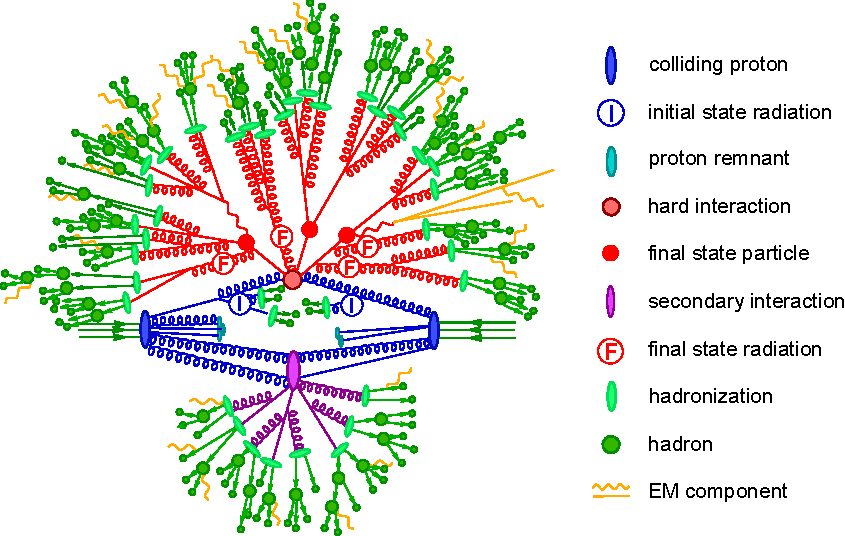
\includegraphics[scale=0.75]{figures/technique/shower.pdf}
}

A brief overview of the programs used for generation and subsequent hadronization of $t$-channel single top quark production is given in the following.

\begin{description}
\item[MadGraph5\_aMC{@}NLO] The \MGAMC program~\cite{Alwall:2014hca} is a merge of the \gls{lo} \MG generator~\cite{Alwall:2011uj} and \AMC into a common framework. It supports the generation of \gls{lo} or \gls{nlo} samples which can be matched to parton showers using the MLM~\cite{Mangano:2006rw} or MC{@}NLO~\cite{Frixione:2002ik} schemes respectively. The latter method produces a certain fraction of events with negative weights (depending on the process) which stem from a subtraction of additional emissions from the \gls{nlo} matrix element to prevent double-counting. 
Multiple samples of events with additional final state partons at matrix element level can also be merged into a combined sample. Here, the overlap with the \gls{ps} is removed through the FxFx merging scheme~\cite{Frederix:2012ps}.

\item[Powheg] The \POWHEG box (versions~1,2)~\cite{Alioli:2010xd} is a program that contains predefined implementations of various processes such as $t$-channel single top quark production~\cite{Alioli:2009je} at \gls{nlo}. It utilizes the so-called \POWHEG method~\cite{Frixione:2007vw} for matching in which the hardest radiation generated from the \gls{me} has priority over subsequent \gls{ps} emissions. This removes the overlap with the \gls{ps} without the generation of negatively weighted events.

\item[CompHEP] The \COMPHEP program (version~4.5)~\cite{Boos:2004kh} can perform calculations of cross sections from Lagrangians at \gls{lo}. In addition, generation of events is also possible such as single top quark production~\cite{Boos:2006af}. Here, an approximation is used by combining events from the $2\to2$ and $2\to3$ processes which reproduces effectively \gls{nlo} corrections.

\item[Pythia] The \PYTHIA program (versions~6,8)~\cite{Sjostrand:2006za,Sjostrand:2014zea} can generate events of various processes at \gls{lo}. It is however famous for its \gls{ps} simulation which can be interfaced with other \gls{lo} and \gls{nlo} event generators to perform subsequent parton showering, hadronization, and the simulation of the underlying event. For hadronization, a phenomenological model is utilized in which one-dimensional strings\footnote{The string model is motivated by the fact that the spatial form of a dipole color field does not extend radially like an \gls{em} field but is instead squeezed to a tube-like form.} connected to partons reflect the color field leading to the creation of additional partons through string branching and finally to the formation of color-neutral singlets.

\item[Herwig++] The \HERWIG program (version~7)~\cite{Bellm:2015jjp} is an \gls{nlo} event generator which is also capable of simulating the showering of partons similar to \PYTHIA. Its hadronization algorithm utilizes a model in which color-connected quarks are spatially kept together in clusters~\cite{Webber:1983if} which is motivated by the ``preconfinement'' of color~\cite{Amati:1979fg}. If the mass of a cluster is sufficiently high it can decay into lighter clusters with a certain probability. In its final step, a cluster decays then into a pair of hadrons.
\end{description}




%##############################################
\section{Top quark reconstruction}
%##############################################

After the reconstruction and selection of analysis objects, a top quark candidate is reconstructed in the presented analyses. Assuming that the top quark decayed leptonically as $\mathrm{t}\to\mathrm{b}\mathrm{W}\to\mathrm{b}\ell\nu$ its energy and momentum is reconstructed by summing the measured 4-momenta of a selected lepton (muon or electron), b-tagged jet, and neutrino candidate. The neutrino candidate itself is reconstructed from the missing transverse energy and the lepton momentum by requiring a W~boson mass constraint of $m_\mathrm{W}=80.4~\GeV$~\cite{Olive:2016xmw} on their invariant mass as

\begin{align}
m_\mathrm{W}^2=\colvec{2}{E_\mathrm{W}}{\vec{p}_\mathrm{W}}^{2}&\overset{!}{=}\left[\colvec{2}{E_{\ell}}{\vec{p}_{\ell}}+\colvec{2}{E_{\nu}}{\vec{p}_{\nu}}\right]^{2}\nonumber\\
&=\underbrace{m_{\ell}^2+m_{\nu}^2}_{\approx 0}+\,2\cdot E_{\ell}\,E_{\nu}-\,2\cdot\colvec{3}{p_{\ell,x}}{p_{\ell,y}}{p_{\ell,z}}\cdot\colvec{3}{p_{\nu,\mathrm{T}}\cdot\cos\phi_{\nu}}{p_{\nu,\mathrm{T}}\cdot\sin\phi_{\nu}}{p_{\nu,z}}. \label{eq:technique-neutrino-pz-eq}
\end{align}

When taking $p_{\nu,\mathrm{T}}$ and $\phi_{\nu}$ from the missing transverse momentum vector $\pvmiss$, this allows to solve for the unknown $p_{\nu,z}$-component of the neutrino candidate momentum. After rearranging, one obtains from Eq.~\ref{eq:technique-neutrino-pz-eq} the quadratic equation

\begin{equation}
0=p_{\nu,z}^2-\frac{2\,\xi\,p_{\ell,z}}{E_{\ell}^{2}-p_{\ell,z}^2}\cdot p_{\nu,z}-\frac{\xi^{2}-E_{\ell}^{2}\,p_{\nu,\mathrm{T}}^2}{E_{\ell}^{2}-p_{\ell,z}^2},\end{equation}

with

\begin{equation}
\xi=\frac{m_\mathrm{W}^2}{2}+p_{\nu,\mathrm{T}}\,p_{\ell,\mathrm{T}}\cdot\cos\big(\phi_\ell-\phi_\nu\big)
\end{equation}

which possesses the solutions

\begin{align}
p_{\nu,z}^{1,2}=\frac{1}{E_{\ell}^{2}-p_{\ell,z}^{2}}\left[\xi\cdot p_{\ell,z}\pm E_{\ell} \sqrt{\xi^2-p_{\nu,\mathrm{T}}^2\big(E_{\ell}^2-p_{\ell,z}^2\big)}~\right]. \label{eq:technique-neutrino-pz}
\end{align}

A detailed derivation and discussion of this result can be found in Ref.~\cite{Chwalek:1416031}. In simulated $t$-channel single-top-quark events this procedure leads to two real solutions for the neutrino $p_{\nu,z}$-component in about 65\% of all events that passed the selection. From the two solutions the one with the smallest absolute $|p_{\nu,z}|$ is chosen which is found to be closest to the true neutrino $p_{z}$ in 63\% of events with real solutions. In the remaining 37\% of events, both real solutions are found to be close together \todo{how close} such that the mistake here by picking the smallest solution is acceptable. If the discriminant in Eq.~\ref{eq:technique-neutrino-pz} becomes negative the solutions are complex. This happens in about 35\% of events and occurs mostly due to the finite \met resolution whereas the negligence of the W~boson mass width and resolution of the lepton momentum are minor effects. The imaginary part of the solutions is removed by requiring that the discriminant vanishes

\begin{equation}
0\overset{!}{=}\xi^2-p_{\nu,\mathrm{T}}^2\big(E_{\ell}^2-p_{\ell,z}^2\big)~
\Rightarrow~ p_{\nu,z}=\frac{\xi\cdot p_{\ell,z}}{E_{\ell}^{2}-p_{\ell,z}^{2}}
\end{equation}

which is equal to setting the transverse W~boson mass $\mtw$ to the W~boson mass itself

\begin{align}
m_\mathrm{W}^2\overset{!}{=}\mtw^2&=(p_{\ell,\mathrm{T}}+p_{\nu,\mathrm{T}})^2-(p_{\ell,x}+p_{\nu,x})^{2}-(p_{\ell,y}+p_{\nu,y})^{2}\\
&=2\,p_{\ell,\mathrm{T}}^2\,p_{\nu,\mathrm{T}}^2\cdot\Big[1-\cos\big(\phi_\ell-\phi_\nu\big)\Big].
\end{align}

Then, the $p_{\nu,x}$ and $p_{\nu,x}$ components are varied and the transverse momentum which minimizes the distance $|\vec{p}_{\nu,\mathrm{T}}-\pvmiss|$ with respect to the measured missing momentum vector is taken as the result. 

\todo{show improvement of MET res in case of complex solutions}

\todo{top quark matching performance
(top pT/eta as function of b-tag in acceptance after selection, b-quark within dR, top within dR)}

%##############################################
\section{Boosted Decision Trees}
%##############################################

Typically, the $t$-channel single-top-quark signal region, defined by one isolated lepton, 2~jets (where one is b-tagged), and significant \met, is found to be still largely contaminated by events from background processes after the event selection. The \glshere{sb} yield ratios are about 13\% and 14\% at 8~and 13~TeV, respectively~\cite{Khachatryan:2014iya,Sirunyan:2016cdg}\todo{update TOP-16-003 when accepted by PRL}. The majority of background events stems from \wjets, \ttbar, and multijet production whereas the contributions from single top tW and $s$-channel, Drell-Yan, and diboson production are minor. The small \gls{sb} ratio motivates the usages \glshere{mva} techniques. In this thesis, \glsplhere{bdt} are employed for event classification as provided by the \gls[]{tmva} framework~\cite{Hocker:2007ht}. They are based on a set of decision trees where each yields a binary output depending on whether an event is signal- or background-like. Their training and how the single decision tree outputs are combined into a one-dimensional discriminant are detailed in the following.

An exemplary decision tree is presented in Fig.~\ref{fig:technique-decisiontree} where sequential selections on observables $x_{i}$ are applied such that the leaf nodes contain either a majority of signal or background events. It is constructed using samples of simulated events for which the desired classification is a priori known~(``superivsed learning'').

\myfigure{\label{fig:technique-decisiontree} A sketch of a decision tree.}{
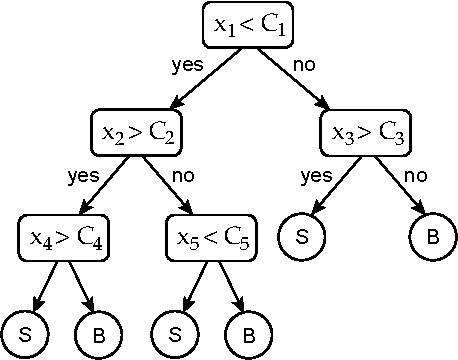
\includegraphics[scale=0.75]{figures/technique/decision_tree.pdf}
}

The optimal observable and working point $C_{i}$ per node are determined by analyzing which set of $(x_{i},C_{i})$ yields the maximal separation between the signal and background distributions. In the analyses, the separation is calculated using the cross entropy 

\begin{equation}
H=-p\cdot\ln(p)-(1-p)\cdot\ln(1-p),\qquad p=N_\mathrm{signal}/N_\mathrm{total}
\end{equation}

where $p$ denotes the achieved purity of a selection. A node is not split further if it contains less than a predefined minimum number of events to ensure that the decisions per node and the binary outputs per leaf are statistically significant. The minimum number of events can be optimized to mitigate potential ``overtraining'' of a decision tree. This occurs when statistical fluctuations are learned instead of the physical distributions due to the finite statistics of the training sample. Furthermore, special caution is required when using a sample which contains also negatively weighted events~(e.g. \MGAMC). If a tree has selected a majority of negatively weighted events in a leaf, any decision would be incorrect since distributions of the selected events are unphysical if they are not countered by sufficient amounts of positively weighted ones. The cancellation of negatively weighted events can be tweaked by increasing the minimum number of events per node beyond the statistical motivated threshold one would choose when training only on a sample of purely positively weighted events.

A single decision tree trained this way can still be perceptible to statistical fluctuation leading to misclassification errors when given a statistically-independent test sample which was not used in the training. This can be mitigated by training multiply decision trees with outputs $h_{i}$ that are then combined using a majority vote as

\begin{equation}
M(\vec{x})=\sum_{i}^{N_\mathrm{trees}}~w_{i}\cdot h_{i}\,(\vec{x};\,\vec{C}_{i})\label{eq:technique-majority-vote}
\end{equation}

where $\vec{x}$ denotes the values of the observables per event and $w_{i}$ are the so-called boosting weights. Another advantage is that the single decision trees only need to be ``weak learners''. This means that they are usually very shallow, e.g. 2 or 3 layers of selections, and provide only a moderate accuracy over random guessing which increases also their robustness against overtraining. By adjusting the weights through a boosting procedure, the accuracy per tree is accounted for in the majority vote. Thus a strong learner is created by combining several weak ones~\cite{Schapire1990,FREUND1995256}. The two boosting procedures employed in this thesis are the adaptive boosting, \ADABOOST~\cite{FREUND1997119}, and \GRADIENTBOOST~\cite{Friedman00greedyfunction} algorithms. In the \ADABOOST algorithm, decision trees are trained iteratively. At each step, a single decision tree is trained and the misclassified events are identified. Their weight is increased in the training of subsequent tree by the boosting weight

\begin{equation}
\alpha_{n+1}=\left(\frac{1-\epsilon_{i}}{\epsilon_{i}}\right)^\beta
\end{equation}

where $\epsilon_{i}$ denotes the misclassification rate of the current tree $i$ and $\beta$ a configurable learning rate. The corresponding weight in Eq.~\ref{eq:technique-majority-vote} is then given by $w_{i}=\ln\alpha_{i}$. Typically a slow learning rate of $\beta\leq0.5$ is chosen to allow for more boosting steps. It can be shown that the \ADABOOST algorithm is equivalent to the minimization of the exponential loss function $L(M,y)=\exp(-M(\vec{x})\,y)$ where $y$ denotes the true classification of the event~\cite{Hocker:2007ht}. If the loss function is changed to 

\begin{equation}
L(M,y)=\ln\left(1+e^{-2\,M(\vec{x})\,y}\right)
\end{equation}

the \GRADIENTBOOST procedure is obtained. This loss function is more robust in the presence of outliers and noise events for which the \ADABOOST algorithm may degrade. In the \GRADIENTBOOST procedure the loss function is iteratively minimized with respect to the weights and decision tree parameters in $M$ using the method of gradient decent. During the minimization, the output of the majority vote gradually tends towards $y$ because misclassified events result in large gradients of the loss function. Similar to the \ADABOOST algorithm, an increased performance is obtained when decreasing the learning rate which is called ``shrinkage'' here. It decreases the parameter updates during the gradient decent minimization. In the analyses, both boosting algorithms have been tested to validate their performances with respect to each other. Only negligible differences in their discrimination power have been found.  \todo{write better?}

The discrimination power of a trained \gls{bdt} is assessed by analyzing the \glshere{roc} curve. Exemplary \gls{roc} curves are presented in Fig.~\ref{fig:technique-bdt-rocs}. The \gls[]{auc} values denote the area under the \gls{roc} curve with respect to random guessing. Here, the \gls{roc} curves of a \gls{bdt} trained to discriminate $t$-channel single-top-quark events against \wjets and \ttbar background events is compared to the pseudorapidity of the untagged light jet and to the reconstructed top quark mass difference. An \gls{auc} of $31\%$ is achieved with the trained \gls{bdt} which outperforms the other two $t$-channel typical observables.\todo{write better?}


\myfigure{\label{fig:technique-bdt-rocs}Comparison of \gls{roc} curves for separating $t$-channel single-top-quark events from background events (\wjets, \ttbar) using: random guessing; a trained \gls{bdt} discriminant; the pseudorapidity of the untagged light jet ($\jprime$); the difference of the reconstructed top quark mass with respect to the nominal mass, $\Delta m_\mathrm{top}=m_\mathrm{top}-172.5~\GeV$.}{
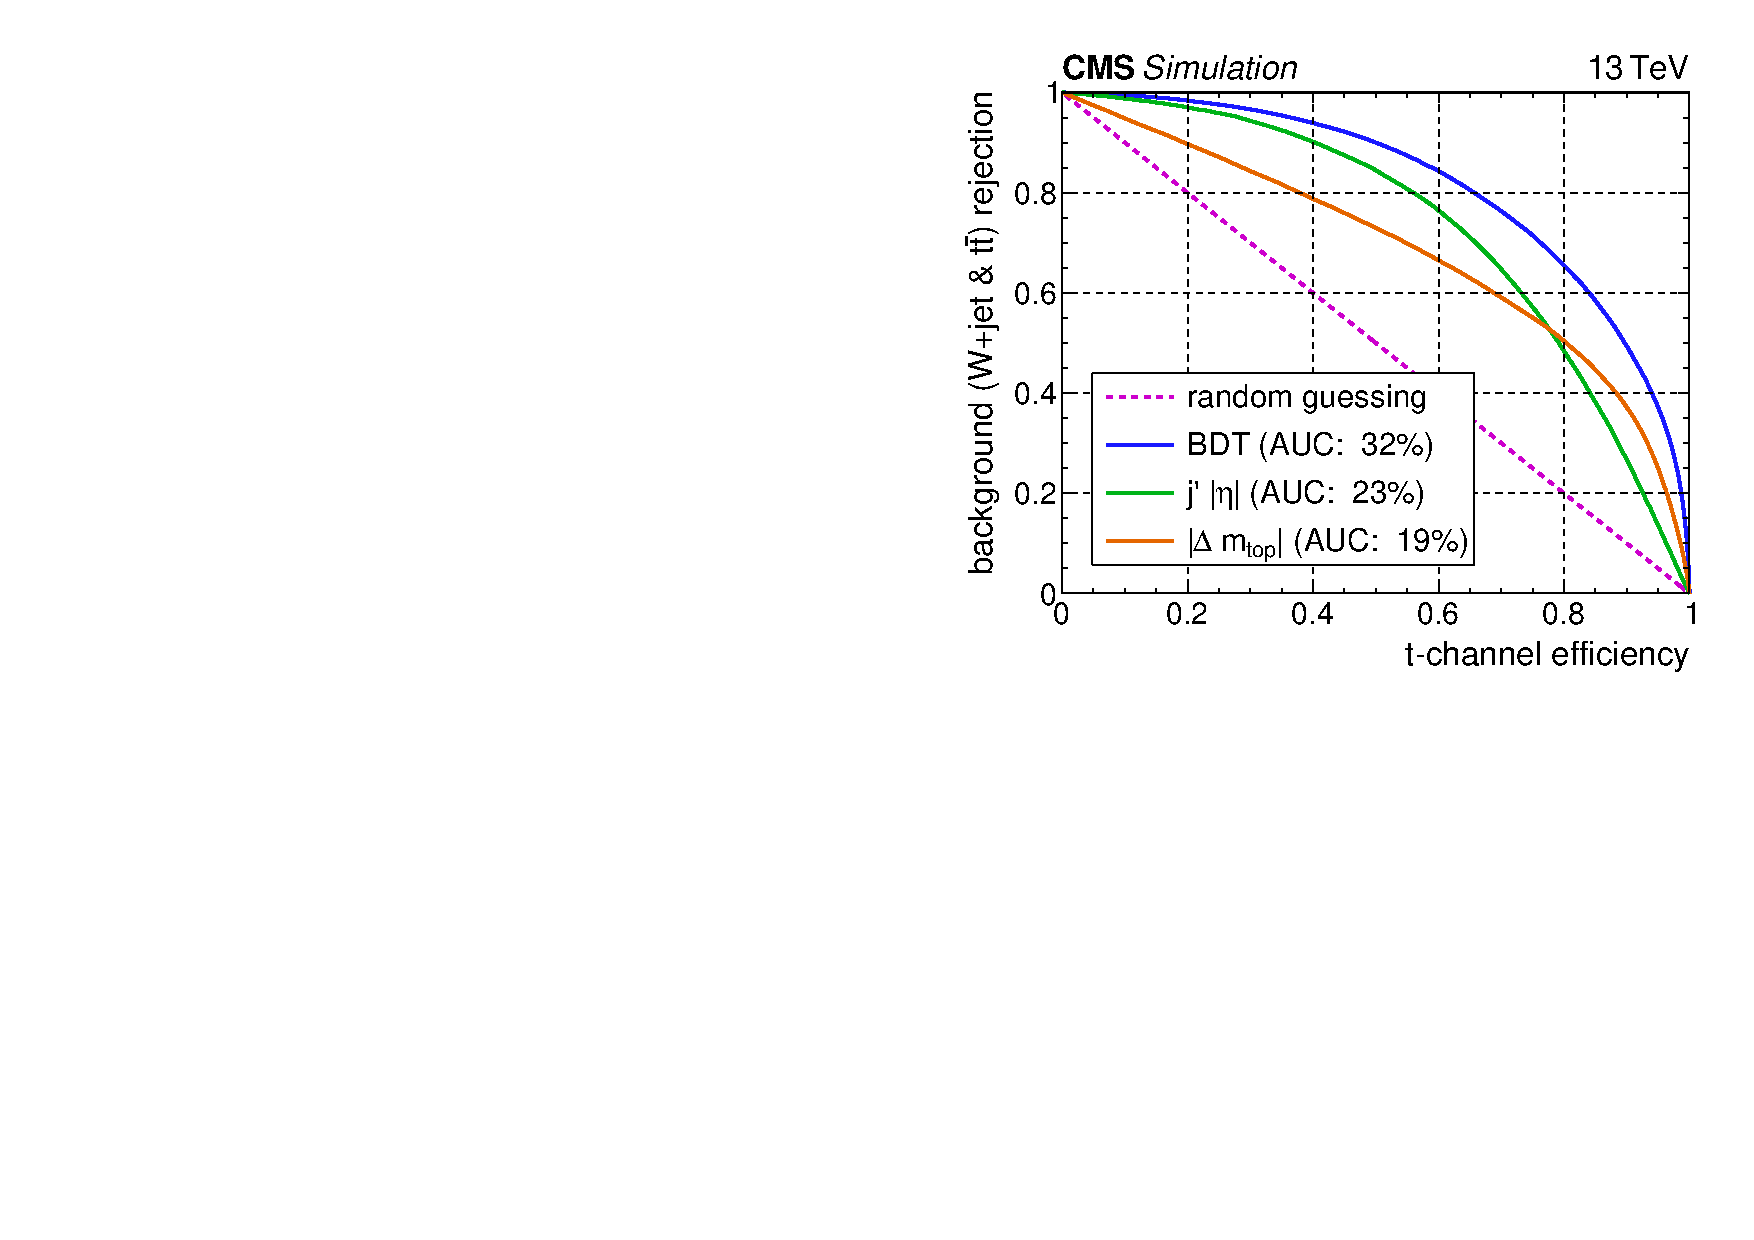
\includegraphics[width=0.6\textwidth]{figures/technique/rocs.pdf}
}


%##############################################
\section{Template-based fitting}
%##############################################

In the analyses, the amount of signal and background events is estimated from data using template-based \glshere{ml} fits. The templates are obtained from simulated events 

likelihood, barlow-beeston method, sys

%##############################################
\section{Partonic and fiducial objects}
%##############################################

dressed leptons (cone algorithms associates photons to leptons but does not cluster close leptons), jet clustering (no neutrinos/leptons), b-tagging

%##############################################
\section{Unfolding}
%##############################################

problems, regularization scheme, correlations, subway plot, alternative FBU
